Los árboles de decisión son modelos de aprendizaje supervisado que se utilizan para predecir a qué clase o categoría pertenece un caso conocido mediante uno o más atributos. Estos modelos se construyen utilizando un algoritmo llamado \emph{partición binaria recursiva}. Durante el entrenamiento, el algoritmo realiza divisiones en un subconjunto de los datos basadas en decisiones asociadas a variables conocidas, generando así dos nuevos subconjuntos. Este proceso se repite de manera recursiva hasta alcanzar un punto de terminación predefinido, lo que resulta en la creación del clasificador basado en árbol de decisión. Luego, cada nuevo dato, que posee atributos conocidos, sigue las ramificaciones del árbol siguiendo las reglas y decisiones generadas durante el proceso de entrenamiento.

En la actualidad, los árboles de decisión son unos de los modelos de aprendizaje más utilizados debido a su buen rendimiento \cite{arboles-decision}. Estos algoritmos pueden generar modelos predictivos tanto para variables cuantitativas (regresión) como para variables cualitativas o categóricas (clasificación).

Como se mencionó anteriormente, un árbol de decisión realiza tareas de clasificación. Un clasificador es un algoritmo que nos permite asignar sistemáticamente una clase a cada uno de los casos presentados.

\begin{figure}[H]
    \begin{minipage}[t]{0.9\textwidth}
        \caption{Estructura de un árbol de decisión}
        \label{arbol-de-decision}        
    \end{minipage}

    \vspace{10pt}

    \begin{minipage}[b]{1.1\textwidth}
        \centering
        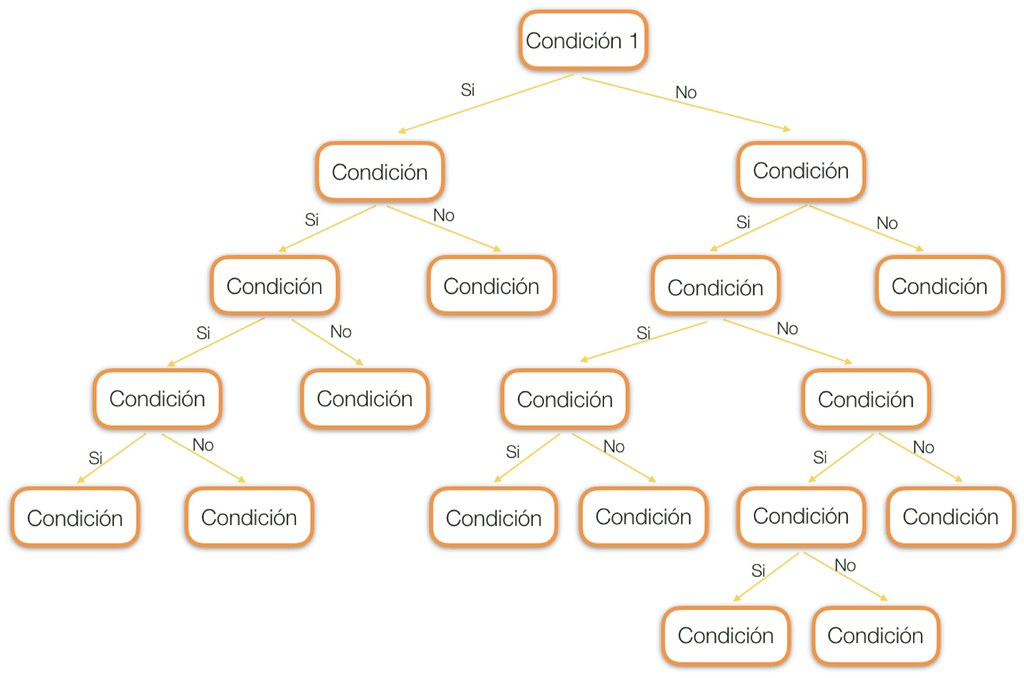
\includegraphics[width=\textwidth]{img/estructura-arbol-de-decision.jpg}        
    \end{minipage}

    \begin{minipage}[t]{0.9\textwidth}
        Fuente: Aprende IA. Recuperado de \url{https://aprendeia.com/arboles-de-decision-clasificacion-teoria-machine-learning/}
    \end{minipage}
\end{figure}

En la figura anterior se puede visualizar la estructura que posee un árbol de decisión, en este se aprecia como actua el algoritmo de partición binaria mencionado al comienzo, tomando un conjunto y separandolo en subconjuntos hasta llegar a un final previamente establecido.

Para estimar la precisión de un clasificador, se calcula la tasa de error de clasificación verdadera. Esta tasa se obtiene evaluando un conjunto de valores X a los que el clasificador asigna una clase incorrecta, y se divide por el total de valores en X. Idealmente, se debería conocer la clase de todos los casos en el universo antes del entrenamiento, o en su defecto, de una muestra de tamaño similar al universo. Sin embargo, en la mayoría de los casos reales, no se dispone de todos los datos del universo, por lo que se trabaja con una muestra y se estima la tasa de error mencionada anteriormente utilizando \emph{estimadores internos}.

\subsubsection{Ventajas de los árboles de decisión}
\begin{itemize}
    \item \textbf{Interpretabilidad:} Los árboles de decisión son fácilmente interpretables y comprensibles para los humanos. La estructura del árbol se puede visualizar de manera intuitiva, lo que permite comprender cómo se toman las decisiones y qué atributos son más relevantes para la clasificación.
    \item \textbf{Facilidad de uso:} La construcción y el uso de un árbol de decisión son relativamente sencillos en comparación con otros algoritmos de aprendizaje automático más complejos. No requieren una preparación exhaustiva de los datos ni un procesamiento previo complicado. Además, los árboles de decisión pueden manejar datos numéricos y categóricos sin requerir transformaciones adicionales, lo que simplifica el flujo de trabajo de modelado.
    \item \textbf{Capacidad para manejar datos faltantes y variables irrelevantes:} Los árboles de decisión tienen la capacidad de manejar datos faltantes en los atributos de forma natural. Durante la construcción del árbol, si un atributo tiene valores faltantes, el modelo puede utilizar otros atributos para tomar decisiones sin requerir imputación de datos. Además, los árboles de decisión son resistentes a variables irrelevantes, lo que significa que pueden ignorar atributos que no aportan información útil para la clasificación.
    \item \textbf{Flexibilidad y robustez:} Los árboles de decisión pueden manejar tanto problemas de clasificación como de regresión. Además, son capaces de capturar relaciones no lineales entre los atributos y la variable objetivo. Aunque cada árbol individual puede ser susceptible al sobreajuste, se pueden aplicar técnicas de regularización, como la poda, para mejorar la generalización y evitar el sobreajuste.
    \item \textbf{Eficiencia en tiempo de entrenamiento y predicción:} Los árboles de decisión tienen tiempos de entrenamiento y predicción rápidos, ya que solo implican la evaluación de una serie de reglas de decisión. Aunque el tiempo de construcción puede ser mayor para conjuntos de datos grandes, una vez construido, el árbol puede ser utilizado eficientemente para hacer predicciones en tiempo real.
\end{itemize}

\subsubsection{Desventajas de los árboles de decisión}
\begin{itemize}
    \item \textbf{Sensibilidad a cambios pequeños en los datos:} Los árboles de decisión son muy sensibles a cambios pequeños en los datos de entrenamiento. Una modificación mínima en los datos de entrada puede dar lugar a un árbol de decisión completamente diferente. Esto puede hacer que el modelo sea inestable y su rendimiento pueda variar significativamente.
    \item \textbf{Tendencia al sobreajuste:} Los árboles de decisión tienen la capacidad de adaptarse demasiado a los datos de entrenamiento. Si no se controla adecuadamente, el árbol puede memorizar el ruido o las fluctuaciones aleatorias en los datos de entrenamiento, lo que puede resultar en un mal rendimiento en datos nuevos y no vistos. La poda y otras técnicas de regularización se utilizan para mitigar este problema.
    \item \textbf{Limitaciones en la representación de relaciones complejas:} Aunque los árboles de decisión pueden capturar relaciones no lineales entre atributos y la variable objetivo, pueden tener dificultades para representar relaciones complejas que requieren una combinación de múltiples atributos. Las decisiones tomadas en cada nodo se basan en un solo atributo, lo que puede limitar su capacidad para modelar interacciones más sofisticadas.
    \item \textbf{Propensión a sesgos en los datos de entrenamiento:} Los árboles de decisión pueden verse afectados por sesgos en los datos de entrenamiento, especialmente cuando hay desequilibrios en las clases o falta representación de ciertas categorías. Esto puede resultar en una clasificación desigual o inexacta en casos minoritarios o poco representados.
\end{itemize}